\chapter{Implementation}
\label{ch:implementation}

\section{Chauffeur Service}

%  \begin{itemize}
%     \item Take some Pictures
%     \item Chauffeur service for German federal agency.
%     \item Takes new Chauffeur Jobs
%     \item UI overview of Jobs, and Jobs Details
%     \item Overview of Chauffeurs and their availability 
%     \item UI to manage Jobs, assign chauffeurs
%     \item group Jobs
%  \end{itemize}

As a basis for our case study we used an application called DSW-FD (Dispositions-software-Fahrdienst). DSW-FD is used to schedule chauffeur rides for a German federal agency. The application provides a rich user interface, with views for managing chauffeur jobs, as well as chauffeur drivers. Clients which need a Chauffeur ride can call a separate hotline, where a handler creates a new chauffeur job, this job is then sent to DSW-FD where it appears in the overview of Jobs, and can then be processed by a Job handler.


\begin{figure}
    \centering
    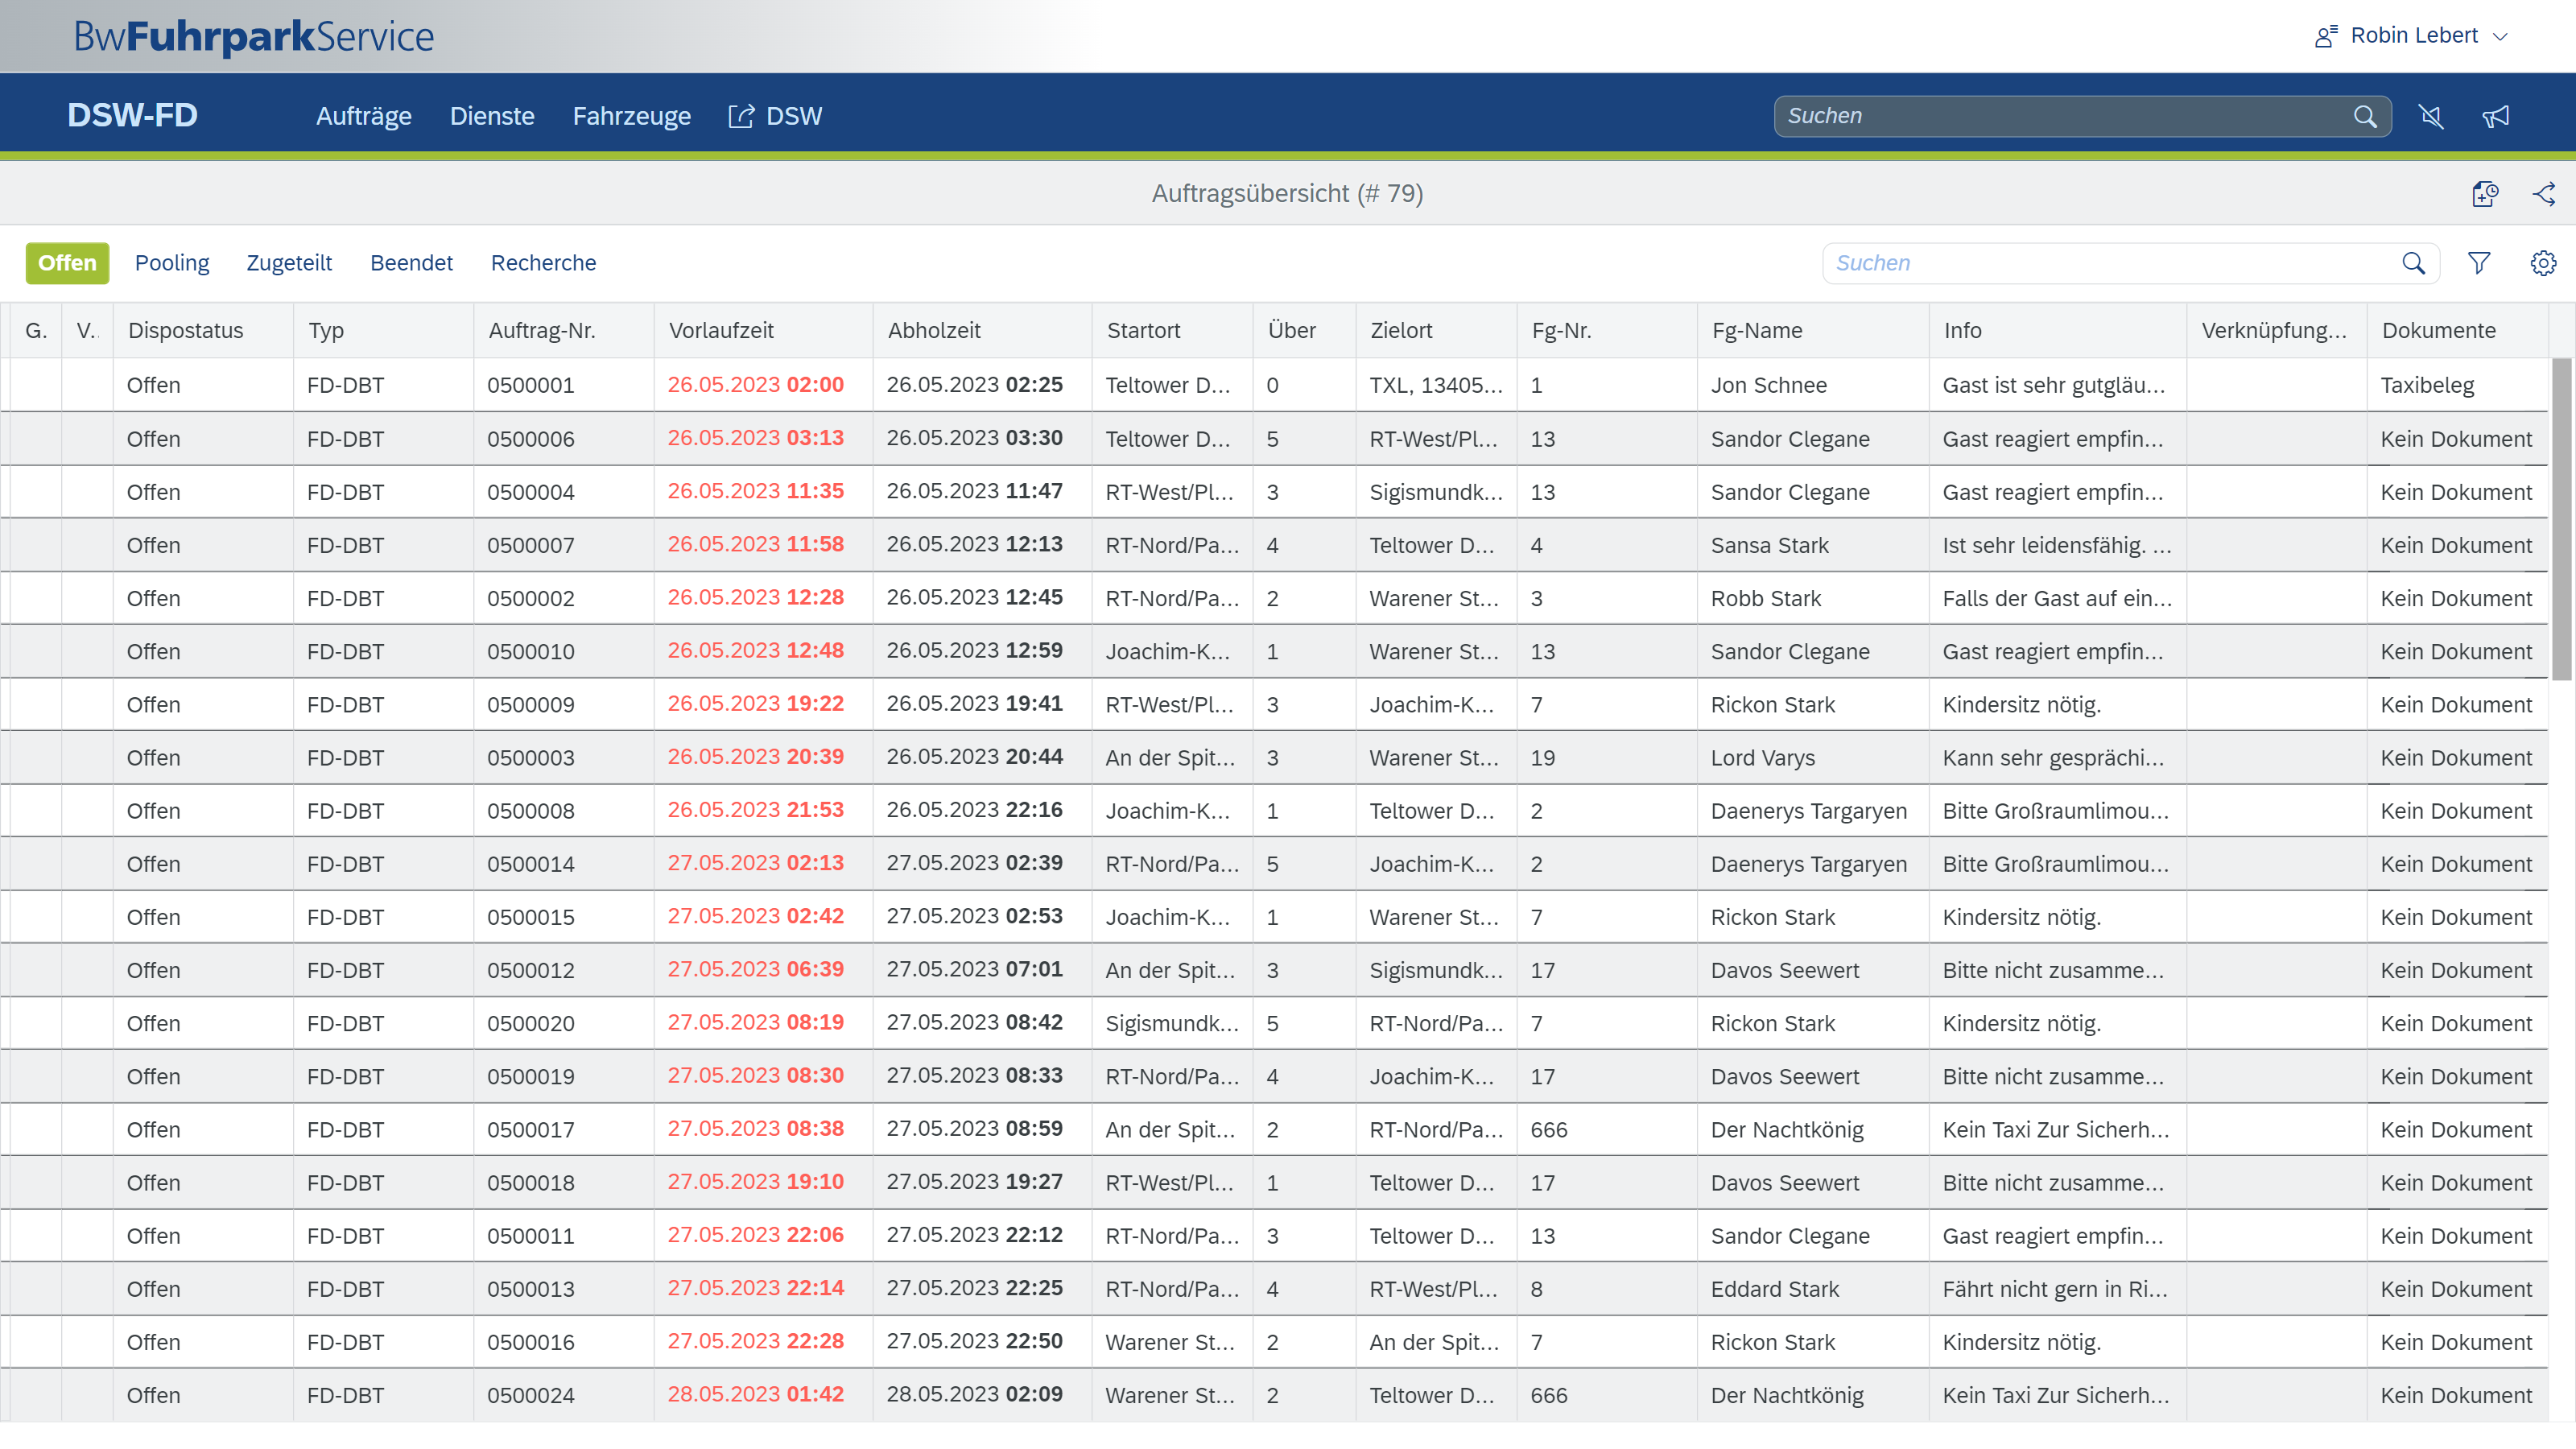
\includegraphics[width=\linewidth]{assets/current-auftrag-overview}
    \caption{Overview of chauffeur jobs in current implementation}
    \label{fig:current-overview-auftrag}
\end{figure}


Drivers need to be manually assigned to a job by a handling person. To this end, the application provides suggestions for drivers which would be free when the job is schedule and are closest to the job's departure point. Furthermore, the app provides functionality to group together different jobs so that they may be handled by a single driver, determine the return destination for the driver after they finished the job, as well as marking a job as being handled by a pool of drivers.

\begin{figure}
    \centering
    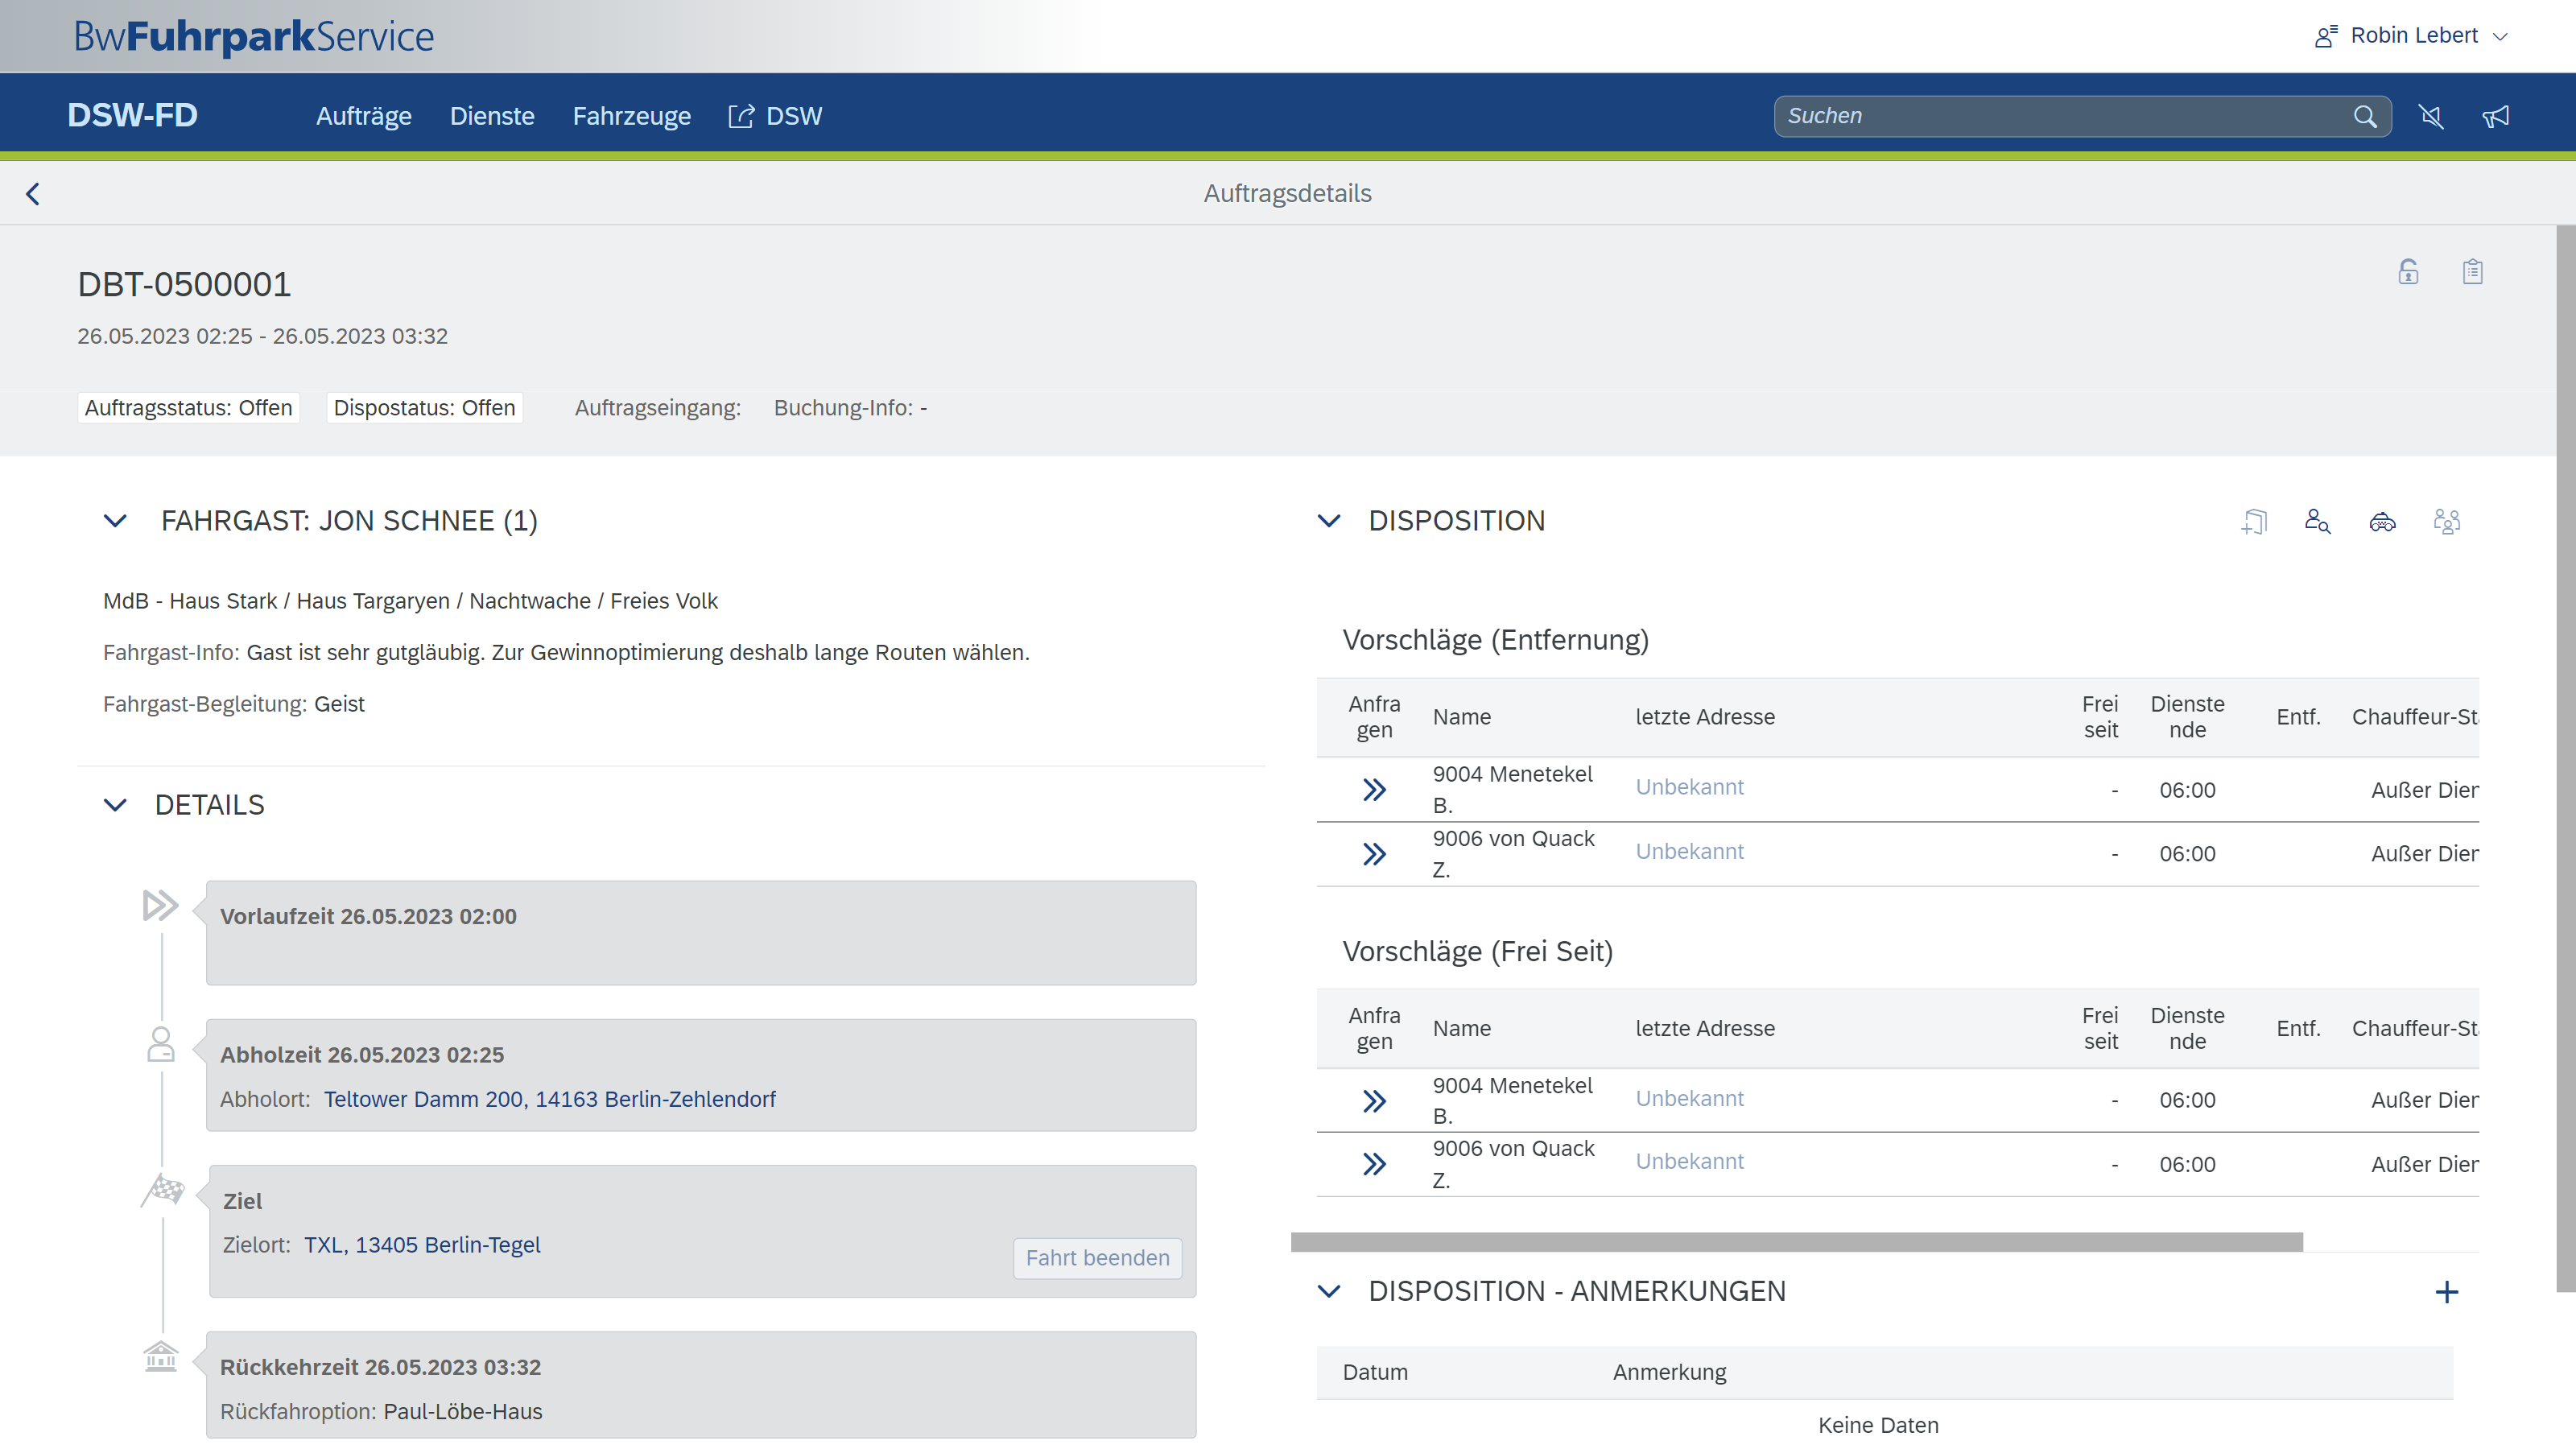
\includegraphics[width=\linewidth]{assets/current-auftrag-details}
    \caption{Chauffeur job details view in current implementation}
    \label{fig:current-details-auftrag}
\end{figure}

The application also provides features to directly interact with drivers, such as broadcasting messages to all drivers, reminding a driver to take their mandatory break, and directly calling a driver.

\section{Current Implementation}

% \begin{itemize}
%     \item UI5-Frontend
%     \item Java-Backend
%     \item Android app for drivers.
%     \item OIDC
%     \item mssql
% \end{itemize}

The current Implementation is realized as a classic frontend, backend architecture. The backend is implemented using the Java framework Spring Boot. It provides a SOAP web server on which new Jobs are submitted. Data is persisted in a MSSQL database. The backend also provides Multiple REST API's and an OData API for communication with the frontend. Furthermore, the backend has to interact with Firebase.

The System provides two frontends, an android application, which is used by the chauffeur drivers to receive jobs and communication from headquarters and a web client which is used by handlers to manage jobs and drivers. The web client is implemented using OpenUI5. OpenUI5 is a frontend framework published by SAP, it is intended to develop enterprise applications which follow SAP's Fiori design guidelines. All APIs of the backend require authentication. To this end the frontend has to authenticate with a Keycloak instance using OpenID Connect (OIDC).

\begin{figure}[ht]
    \centering
    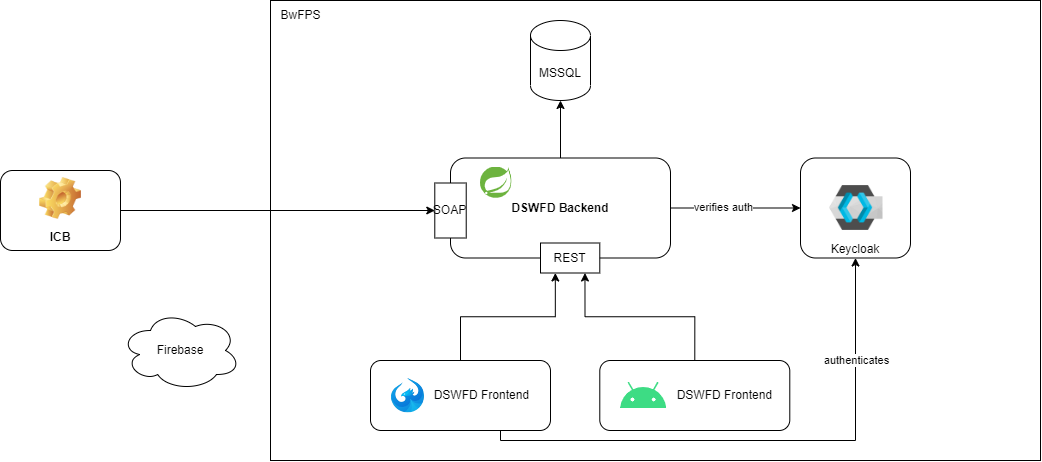
\includegraphics[width=.8\linewidth]{assets/dswfd-architecture}
    \caption{Architecture overview of the current implementation}
    \label{fig:dswfd-architecture}
\end{figure}

\section{SvelteKit Implementation}

% \begin{itemize}
%     \item Two approaches (full stack, FE only)
%     \item First try UI5 web components, second try CSS classes
%     \item Authentication
% \end{itemize}

We experimented with two different implementations. One where SvelteKit replaces Backend and frontend and one where SvelteKit only replaces the Frontend.

\subsection{Full Stack Implementation}

% \begin{itemize}
%     \item prisma 
%     \item easier Authentication
% \end{itemize}

For the full stack implementation SvelteKit has to replace frontend as well as backend, to this end business logic, database communication and API's all have to be implemented in SvelteKit. We used Prisma \cite{noauthor_prisma_nodate} as an ORM to communicate with the database, because Prisma provides functionality to generate its data model from an existing database through introspection. This allowed us to save time on defining models. 


\begin{figure}[ht]
    \centering
    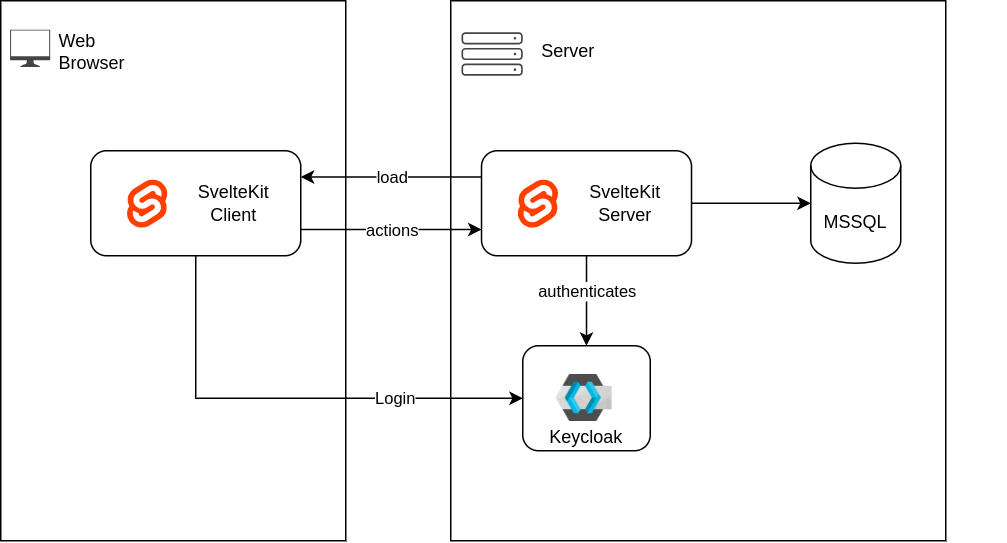
\includegraphics[width=.8\linewidth]{assets/dswfd-architecture-fullstack}
    \caption{Architecture overview of the implementation using SvelteKit both as frontend and as backend}
    \label{fig:dswfd-architecture-fullstack}
\end{figure}

\subsection{Frontend Implementation}

% \begin{itemize}
%     \item Experimented with direct communication to backend.
%     \item Using universal load functions
%     \item load on server during SSR,
%     \item then client takes over.
%     \item approach would make it possible to run app in SPA mode
          
%     \item Also tried to route all client requests through SvelteKit backend
%     \item easier because use of locales makes authentication simpler and no problems with custom fetch
%     \item enables usage of form actions, otherwise SvelteKit does not really provide any help with post requests.
% \end{itemize}

We also decided to explore an approach where SvelteKit is only used as a frontend. This approach provides more flexibility, as backend technology can be chosen individually. Communication to the backend is primarily handled using Web API's. In our use case we decided to reuse the existing Java backend. The backend's REST API could be queried from SvelteKit. As REST APIs are a something which can be called from frontend and backend, this approach can make use of SvelteKit's universal load functions (\ref{sec:sveltekit-loading}). This means that the backend is only used for fetching, during SSR. After the browser has loaded the page, universal load functions are executed client-side and thus the client redirects its requests directly to the backend, instead of sending  a request to the SvelteKit server, which then requests the data, from the backend, overall saving one step of indirection. If loss of SSR is acceptable, this approach would also make it possible to run the application as an SPA, forgoing dedicated SvelteKit server code. This can be useful, as it allows for the SvelteKit application to be served as static files from a web directory or similar. 

\begin{figure}[ht]
    \centering
    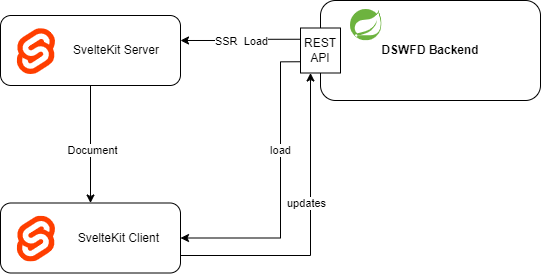
\includegraphics[width=.6\linewidth]{assets/fe-only-client-takes-over}
    \caption{Architecture overview of the implementation using SvelteKit only as a frontend}
    \label{fig:dswfd-architecture-fe-only}
\end{figure}

One problem we encountered with this approach was, that SvelteKit provides no help for sending data to the backend. While data loading is streamlined through universal load functions. Server actions, as used in the full stack implementation, can only be used server side. This means, that implementation for submitting data has to be implemented manually. One way this can be done, is by using the form enhance action which is used to progressively enhance form actions (see \ref{sec:sveltekit-server-actions}):

\begin{myminted}{svelte}{}
<script>
    async function handleSubmit({cancel, request}) {
        cancel();

        const res = await fetch('api/update', {
            method: 'POST',
            body: request.body
        });

        if (!res.ok) {
            // error handling...
        }

        return ({ update }) => {
            update();
        }
    }
<script>

<form method="POST" use:enhance={handleSubmit}>
    <button type="submit">send</button>
</form>
\end{myminted}

It has to also be noted, that forgoing the usage of server actions will mean, that data submission will never work without JavaScript, because the form enhance action can only run when JavaScript is enabled. Instead, the form will make a request to the backend, which then will probably return an error because it is not configured to handle post request.

During this approach we also realized further complications. Firstly, authentication with the backend API becomes more complex, because both client and server need the access token for the API. 
% could this be fixed by passing through the api token??

Furthermore, Svelte's custom fetch function further increased complexity. SvelteKit's implementation of fetch makes sure that fetch behaves similarly on the client and server. Therefore, it enables relative URL paths on the server, which would ordinarily not be possible.

When a page with a universal load function is accessed, the load function is first run on the server during SSR, and the result is sent to the client. During hydration on the client side, the load function is then run again. This means, that ordinarily all fetch calls executed in the load function would run two times, once on the server and once on the client. To prevent this, SvelteKit's implementation inlines fetch responses on the server side, and then uses the inlined response on the client during hydration. This means, that it is necessary to use SvelteKit's fetch implementation. But, as this special fetch function is only exposed as an argument in load functions, one has to always pass this fetch function on any delegates, which require network communication. Furthermore, it is not possible to use custom HTTP-clients, such as Axios\footnote{\url{https://axios-http.com/}}.  

\subsubsection{redirect through server}

To amend these issues we further experimented with an implementation where we only used server load functions and server actions. This implementation is very similar to the full stack implementation discussed earlier. But instead of implementing business logic and database access in the SvelteKit server sided code, the server side is primarily used as middleware that sends REST requests to the Java backend.

\begin{figure}[ht]
    \centering
    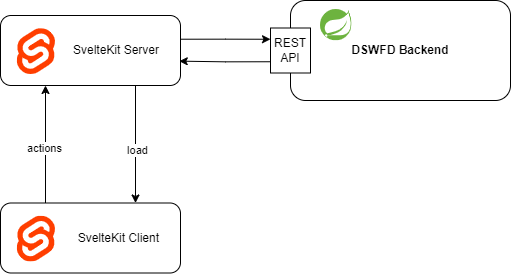
\includegraphics[width=.6\linewidth]{assets/fe-only-all-server}
    \caption{Architecture overview of the implementation using SvelteKit only as a frontend}
    \label{fig:dswfd-architecture-fe-through-server}
\end{figure}

This approach has multiple advantages. It uses much of the in built functionality of SvelteKit, applications can be progressively enhanced, the client requires fewer dependencies, because functionality such as parsing and validating form data can be handled server side. Furthermore, authentication is simplified, as only the backend needs to communicate with the API. And finally, the outlined problems with fetch in universal load functions is solved, because only the backend uses fetch.


\subsection{UI considerations}

The user interface is required to follow the SAP Fiori design guidelines. Our first approach was to use SAP's UI5 Web components. Web components promise to be a framework-agnostic approach to UI components. But we encountered some problems early on:

\begin{itemize}
    \item For now, web components can not be server-side rendered. This is because web components rely on API's which only exist in the browser
    \item Web Components also require JavaScript (at least until \cite{noauthor_declarative_2023})
    \item Problems: Layout shifting, flash of unstyled content ("FOUC")
\end{itemize}
